\cotefile{157-2}
\scanpage{338}
\mspage{77}
% archive sheet number: 337
À la page 61, j'ai invoqué l'existence d'un \uline{foncteur} de ``\uline{composition des chemins}''
\[
\underline{\mathrm{Ch}}_{\Sigma}(X;a,b)\times\underline{\mathrm{Ch}}_{\Sigma}(X;b,c)\mathrel{\unsure{-|\longrightarrow}}\underline{\mathrm{Ch}}_{\Sigma}(X;a,c),
\]
qui sur les fibres du premier \unsure{mb} au dessus de $(\tau,\tau')\in\mathrm{Ob}(\underline{\mathrm{Ty}}\times\underline{\mathrm{Ty}})$, serait donné par
\[
\underline{\mathrm{Ch}}_{\Sigma,\tau}(X;a,b)\times\underline{\mathrm{Ch}}_{\Sigma,\tau'}(X;b,c)\longrightarrow\underline{\mathrm{Ch}}_{\Sigma,\tau\tau'}(X;a,c),\tag*{$(\unsure{*})$}
\]
la composition des chemins de types précisés $\tau,\tau'$. Qu'on ait là un \uline{foncteur}, pas seulement une application sur les ensembles d'objets, est assez évident, et peut s'exprimer par exemple à l'aide du diagramme d'amalgamation
\diagram{\begin{tikzcd}[ampersand replacement=\&,row sep=small,column sep=small]
\& \unsure{\varepsilon|E}=\{0,1\}\arrow[dl,hook]\arrow[dr,hook'] \&\\
I_{\tau}\arrow[dr,hook] \& \& I_{\tau'}\arrow[dl,hook',no head]\\
\& I_{\tau\tau'} \&
\end{tikzcd}}
en le transformant par $\underline{\mathrm{Hom}}(\bullet,X)$ (au lieu de lui \deleted{\unsure{appliquer}} transformer par $\mathrm{Hom}_{\mathrm{Cat}}(\cdot,X)$ seulement), \deleted{\unsure{bien sûr pour la catégorie}} \inserted{du moins dans le cas} particulier où $\Sigma=\mathrm{Fl}(X)$ (qui était celui de la p. 61). Mais le passage aux flèches est assez évident -- pour deux composés
\diagram{\begin{tikzcd}[ampersand replacement=\&,column sep=large,row sep=small]
a\arrow[r,"c_1",""{name=A,below}]\arrow[d,phantom,"\shortparallel" description] \& b\arrow[r,"{c'_1}",""{name=B,below},dash]\arrow[d,phantom,"\shortparallel" description] \& c\arrow[d,phantom,"\shortparallel" description]\\
a\arrow[r,"c_2",""{name=C,above}] \& b\arrow[r,"{c'_2}",""{name=D,above}] \& c
\arrow[from=A,to=C,Rightarrow,"{\unsure{w|u}}"']
\arrow[from=B,to=D,Rightarrow,"{w'}"]
\end{tikzcd}}
$c'_1\circ c_1$ et $c'_2\circ c_2$, de sorte que les hom \inserted{$\unsure{w''|w^{4}}$} du premier dans le \unsure{second}, dans $\underline{\mathrm{Ch}}_{\Sigma}(X;a,c)$, \deleted{``\unsure{sont exactement les couples}} \inserted{\unsure{qui|font} \unsure{sont|sur} l'\unsure{identité|identific$^{\mathrm{tion}}$} sur le sommet} d'indice $n+1$ des \inserted{deux} chemins (où $n=\mathrm{long}\,\tau$), \unsure{correspondant|correspond} à \deleted{\unsure{$\mathrm{id}_{\Sigma,\tau}$}} \unsure{$1_{\tau}$} et à \unsure{$0_{\tau'}$}, ``sont'' exactement les couples
\scanpage{339}
\mspage{78}
% archive sheet number: 338
formés d'un hom $\unsure{w|u}:c_1\to c_2$ et $w':c'_1\mathrel{\unsure{-|\to}}c'_2$ dans $\underline{\mathrm{Ch}}_{\Sigma,\tau}(a,b)$ et $\underline{\mathrm{Ch}}_{\Sigma,\tau'}(b,c)$ respectivement, et si $w'',w,w'$ se correspondent ainsi, on posera
\[
w''=w*w'.
\]

(Il y a une transitivité évidente à vérifier pour voir que ça définit un \uline{foncteur} $\unsure{(*)}$. On peut exprimer la situation à l'aide du diagramme
\diagram{\begin{tikzcd}[ampersand replacement=\&,row sep=large,column sep=small]
\& \underline{\mathrm{Ty}}\times \underline{\mathrm{Ty}}\arrow[rr,"{\Pi\;(\text{composition})}"]\arrow[dl,"p_1"']\arrow[dr,"p_2"] \& \& \underline{\mathrm{Ty}}\\
\underline{\mathrm{Ty}} \& \& \underline{\mathrm{Ty}} \& {,}
\end{tikzcd}}
où $p_1,p_2$ sont les deux projections. On considère sur $\underline{\mathrm{Ty}}\times \underline{\mathrm{Ty}}$ les trois catégories fibrées
\[
p_1^*(\underline{\mathrm{CH}}_{\Sigma,\tau}(a,b)),\quad
p_2^*(\underline{\mathrm{CH}}_{\Sigma,\tau'}(b,\unsure{c})),\quad
\Pi^*(\underline{\mathrm{Ch}}_{\Sigma,\tau\tau'}(a,c))
\]
dont les fibres en $(\tau,\tau')$ sont respectivement
\[
\underline{\mathrm{Ch}}_{\Sigma,\tau}(a,b),\quad
\underline{\mathrm{Ch}}_{\Sigma,\tau'}(b,c),\quad
\underline{\mathrm{Ch}}_{\Sigma,\tau\tau'}(\unsure{\text{à}|a},c).
\]

(On \unsure{a} écrit $\underline{\mathrm{CH}}$ au lieu de $\underline{\mathrm{Ch}}$, pour indiquer que l'on considère les catégories envisagées comme des catégories (fibrées) \uline{au dessus de} $(\underline{\mathrm{Ty}})$.)
% slanted
\margin{Mais il s'agit pour $p_1^*,p_2^*$ et $\Pi^*$ de produits cartésiens ordinaires vus dans $\mathrm{Cat}$, il n'y a pas \unsure{à avoir|à voir|raison} pour \unsure{cela} à écrire des ``$\mathrm{CH}$''\dots}

Au dessus de $\underline{\mathrm{Ty}}\times \underline{\mathrm{Ty}}$, on a un \deleted{\unsure{foncteur}} (cartésien) de catégories fibrées \deleted{sur $\underline{\mathrm{Ty}}\times$}
\[
p_{\unsure{1|2}}^*\underline{\mathrm{CH}}_{\tau}(a,b))\underset{\underline{\mathrm{Ty}}\times \underline{\mathrm{Ty}}}{\times}
p_2^*(\underline{\mathrm{CH}}_{\tau}(b,c))\longrightarrow\Pi^*(\underline{\mathrm{CH}}_{\tau}(a,c)),\tag*{$(**)$}
\]
\scanpage{340}
\mspage{79}
% archive sheet number: 339
car c'est OK sur les fibres ($( * )$ page 77), et si
\[
(\varphi,\varphi'):(\tau_1,\tau'_1)\longrightarrow(\tau,\tau')\qquad
(\varphi:\tau_1\to\tau,\;\varphi':\tau'_1\mathrel{\unsure{-|\to}}\tau')
\]
est une flèche de $\underline{\mathrm{Ty}}\times\underline{\mathrm{Ty}}$, on en déduit un diagramme commutatif \deleted{\unsure{de}}
\diagram{\begin{tikzcd}[ampersand replacement=\&,column sep=large,row sep=large]
\underline{\mathrm{Ch}}_{\Sigma,\tau}(a,b)\times\underline{\mathrm{Ch}}_{\Sigma,\tau'}(b\unsure{;|,}c)
\arrow[r,"{\mathrm{comp.}}"]\arrow[d,"{\varphi_{a,b}^*}"',"{\times}" description,"{{\varphi'}_{bc}^*}"]
\&\underline{\mathrm{Ch}}_{\Sigma,\tau}(a,c)\arrow[d,"{(\varphi*\varphi')_{a,c}^*}"]\\
\underline{\mathrm{Ch}}_{\Sigma,\tau_1}(a,b)\times\underline{\mathrm{Ch}}_{\Sigma,\tau'_1}(b,c)
\arrow[r,"{\mathrm{comp}}"]\&\underline{\mathrm{Ch}}_{\Sigma,\tau_1\tau'_1}(a,c){,}
\end{tikzcd}}
i.e. la composition des chemins \deleted{\unsure{est co}} d'extrémités fixées est compatible avec les images inverses de chemins par\unsure{.|,} \deleted{\unsure{morphismes sur}} \inserted{flèches entre} les types \unsure{des|de} chemins.

Mais l'hom \inserted{cartésien $(**)$} de catégories fibrées sur $\underline{\mathrm{Ty}}\times\underline{\mathrm{Ty}}$ n'est pas tout à fait la $=$ chose qu'un véritable foncteur
\[
\underline{\mathrm{Ch}}_\Sigma(a,b)\times\underline{\mathrm{Ch}}_\Sigma(b,c)\longrightarrow\underline{\mathrm{Ch}}_\Sigma(a,c).\tag*{$(*)$}
\]

La formule $(*)$ \deleted{\unsure{la}} définit en tout cas une application sur les ensembles d'objets, puisque \inserted{les ens. d'objets de} chacune des trois catégories envisagées se décompose en somme \unsure{d'ens|de ceux} $\mathrm{Ch}_{\Sigma,\tau}(\bullet,\bullet)$, où $\tau$ parcourt $\mathrm{Ty}=\mathrm{Ob}\,\underline{\mathrm{Ty}}$. Mais cel\unsure{a} se prolonge-t-il de façon naturelle aux morphismes~? \deleted{Il faut donc se donner encore un \deleted{\unsure{morphisme}} \inserted{flèche} \unsure{dans|de} $\underline{\mathrm{Ch}}_\Sigma(a,b)$, $\varphi:\tau_1\longrightarrow$}
\scanpage{341}
\mspage{80}
% archive sheet number: 340
\deleted{une autre \unsure{dans|de} $\underline{\mathrm{Ch}}_\Sigma(b,c)$, ce qui conduit (en regardant leurs images dans $\underline{\mathrm{Ty}}$) à se donner \unsure{encore}}
\deleted{\[
\varphi:\tau_1\longrightarrow\tau,\qquad\varphi':\tau'_1\mathrel{\unsure{-|\to}}\tau'\qquad\text{dans }\underline{\mathrm{Ty}},
\]}
\deleted{deux \inserted{couples d'}objets $(c,c'),(c_1,c'_1)$ de $\underline{\mathrm{Ch}}_{\Sigma,\tau}(a,b)\times\underline{\mathrm{Ch}}_{\Sigma,\tau'}(b,c)$ et de $\underline{\mathrm{Ch}}_{\Sigma,\tau_1}(a,b)\times\underline{\mathrm{Ch}}_{\Sigma,\tau'_1}(b,c)$ respectivement et des hom}
\deleted{\[
\left\{\begin{aligned}
c_1&\overset{\unsure{w|u}}{\mathrel{\unsure{-|\longrightarrow}}}\varphi^*(c) \qquad\text{\unsure{de}}\\
c'_1&\xrightarrow{w'}{\varphi'}^*(c')
\end{aligned}\right.
\]}
\deleted{et on voudrait en déduire une flèche de $\underline{\mathrm{Ch}}_{\Sigma,\deleted{\unsure{\tau\tau'}}}(a,c)$ au dessus de la flèche \deleted{$\varphi'*\varphi:\tau$}}
\deleted{\[
\varphi'*\varphi:\tau'_1*\tau_1\longrightarrow\tau'\cdot\tau.
\]}

\deleted{Mais voilà que}

Mais voilà que je me rappelle que ce fameux produit cartésien $p_1^*(\text{\unsure{fourbi}})\times p_2^*(\text{\unsure{machin}})$ n'est autre que le produit cartésien tout bête
\[
\underline{\mathrm{Ch}}_\Sigma(a,b)\times\underline{\mathrm{Ch}}_\Sigma(b,c),
\]
envoyé sur $\underline{\mathrm{Ty}}\times\underline{\mathrm{Ty}}$ par le produit cartésien des deux foncteurs de projection
\[
\begin{aligned}
p_{a,b}:{}&\underline{\mathrm{Ch}}_\Sigma(a,b)\longrightarrow\mathrm{Ty}\\
p_{b,c}:{}&\underline{\mathrm{Ch}}_\Sigma(b,c)\longrightarrow\mathrm{Ty},\qquad\text{d'où}
\end{aligned}
\]
\diagram{\begin{tikzcd}[ampersand replacement=\&]
\mathrm{Ch}_\Sigma(a,b)\times\underline{\mathrm{Ch}}_\Sigma(b,c)\arrow[d,"{p_{a,b}\times p_{b,c}}"]\\
\underline{\mathrm{Ty}}\times\underline{\mathrm{Ty}}
\end{tikzcd}}
\scanpage{342}
\mspage{81}
% archive sheet number: 341
qui est bel et bien fibrant (comme produit cartésien de deux foncteurs fibrants) et a les fibres qu'il faut~! On trouve donc bien, par le \unsure{sorite} général sur les foncteurs fibrants (ici sur $\underline{\mathrm{Ty}}\times\underline{\mathrm{Ty}}$) \unsure{une|un} foncteur de catégories fibrées sur $\underline{\mathrm{Ty}}\times\mathrm{Ty}$
\diagram{\begin{tikzcd}[ampersand replacement=\&,row sep=small,column sep=small]
\underline{\mathrm{Ch}}_\Sigma(a,b)\times\underline{\mathrm{Ch}}_\Sigma(b,c)\arrow[r] \& \Pi^*(\mathrm{CH}_\Sigma^{\unsure{\prime}}(a,c))\arrow[d,equal]\\
\&(\underline{\mathrm{Ty}}\times\underline{\mathrm{Ty}})\underset{\underline{\mathrm{Ty}}}{\times}\underline{\mathrm{Ch}}_\Sigma(a,c)\arrow[dl,shorten <=2pt]\\
\text{produit fibré \unsure{pour|par} }\Pi:\underline{\mathrm{Ty}}\times\underline{\mathrm{Ty}}\to\underline{\mathrm{Ty}}\&
\end{tikzcd}}

Comme on a d'autre part un \deleted{\unsure{morphisme}} foncteur du dernier membre (produit fibré) vers \unsure{le} facteur $\underline{\mathrm{Ch}}_\Sigma(a,c)$, on gagne. (On l'aurait \unsure{retrouvé|retrouvée} par le raisonnement direct que je m'apprêtais à faire, et que j'ai biffé -- mais je suis plus heureux comme ça~!)

Pour bien faire, il faudrait prouver l'\uline{associativité} des foncteurs de composition, pas seulement au niveau des objets, par des arguments comme ceci, mais ça revient simplement à une relation du type
\[
(\unsure{w|u}''\mathbin{\unsure{\circ|*}}w')*w^{\unsure{4|\prime}}=w''*(w'*w)
\]
pour \deleted{\unsure{des}} un système de trois flèches de
\[
\underline{\mathrm{Ch}}_\Sigma(a,b),\quad \underline{\mathrm{Ch}}_\Sigma(b,c)\quad\text{et}\quad\underline{\mathrm{Ch}}_\Sigma(c,d)
\]
respectivement. Ça ne peut être que trivialement
\scanpage{343}
\mspage{82}
% archive sheet number: 342
vrai, mais fastidieux à expliciter.

Les sueurs froides sont terminées~!

En résumé, le formalisme de \inserted{$\underline{\mathrm{Ch}}_\Sigma(X)$ et de} $\underline{\mathrm{Ch}}_\Sigma(X;a,b)$ développé jusqu'à présent donne satisfaction complète sur les points suivants~:

a) Bon formalisme de composition des chemins (qui était dégueulasse avant)

b) Traitement élégant de la construction des catégories de fractions $\deleted{\unsure{X}}{\unsure{M|X}}\Sigma^{-1}$. Mais je m'attends \unsure{que} ce sera moins joli qu'avant, quand il s'agira de remplacer un $(\deleted{X}M,\Sigma)$ par des
\[
\underset{\substack{\shortparallel\\\underline{\mathrm{Hom}}(X,M)}}{M(X)},\Sigma_X
\]
($X$ une catégorie d'indices). C'est pour y pallier qu'il \inserted{me} faudra développer des énoncés de comparaison, entre la catégorie $\underline{\mathrm{Ch}}_\Sigma$ \unsure{construite|construit} ici, et d'autres \unsure{\textsuperscript{$q$}} dont le type dans $\mathrm{Hot}$ se prête aux calculs de façon plus directe, comme dans l'état premier de la question.

De plus, on sera sûrement obligé d'en venir à des Ind-catégories, pour pouvoir \unsure{sauver|suivre} la \unsure{variance} de $M(X)\Sigma_X^{-1}$ pour $X$ variable.

c) Bon formalisme des ``homotopies'' et des compositions d'homotopies (ce qui est une autre façon de parler de chemins et de leur composition).
\scanpage{344}
\mspage{83}
% archive sheet number: 343

\uline{8}. \uline{Le lemme} d'\uline{homotopie pour les morphismes d'intervalles}

C'est le suivant

\uline{Lemme 1} Soient $\tau,\tau'\in\mathrm{Ty}$, et $f,g:\tau\rightrightarrows\tau'$ deux morphismes de $\underline{\mathrm{Ty}}$. Alors $f,g$ sont homotopes dans la catégorie $\underline{\mathrm{Hom}}\,\underline{\mathrm{int}}(I_\tau,I_{\tau'})$ des morphismes (croissants) d'intervalles orientés de $I_\tau$ dans $I_{\tau'}$.

Cette catégorie pourrait \unsure{licitement|librement} se désigner par $\underline{\mathrm{Hom}}_{\underline{\mathrm{Ty}}}(\tau,\tau')$, ou $\underline{\mathrm{Hom}}(\tau,\tau')$. C'est une sous-catégorie \deleted{pleine} de la catégorie $\underline{\mathrm{Hom}}(I_\tau,I_{\tau'})$ de \uline{tous} les foncteurs de $I_\tau$ dans $I_{\tau'}$, et une sous-catégorie pleine de la catégorie $\underline{\mathrm{Hom}}^{\unsure{\varepsilon|E}}(I_\tau,I_{\tau'})$ des foncteurs \inserted{$f$} qui sont compatibles avec les données de \unsure{sources|source} et de \unsure{buts|but}, i.e. qui rendent \unsure{commutatif|commutatifs} le diagramme
\diagram{\begin{tikzcd}[ampersand replacement=\&,column sep=small]
\&\varepsilon=\{0,1\}\arrow[dl,hook,"{(\sigma_\tau,\beta_\tau)}"']\arrow[dr,hook,"{(\sigma_{\tau'},\beta_{\tau'})}"]\&\\
I_\tau\arrow[rr,"f"]\&\&I_{\tau'}
\end{tikzcd}}

Si $f,g$ \deleted{\unsure{ont}} sont dans cette catégorie, \deleted{alors} (qui soient morphismes croissants d'ailleurs), une flèche de $f$ dans $g$ est donc \deleted{\unsure{un hom}} la donnée, pour tout $i\in I_\tau$, d'une \deleted{\unsure{hom}} \inserted{flèche} $f(i)\xrightarrow{\unsure{w|u}_i}g(i)$ de $I_{\tau'}$, \unsure{que|pour|sous} les deux conditions a) si $i\in\{0_\tau,1_\tau\}$, $\unsure{w'|w^{i}}=\mathrm{id}$ et b) le carré commutatif habituel pour une flèche $i\to j$ de $I_\tau$. (\unsure{Il} suffit d'avoir cette compatibilité pour les flèches de transition $\underline{u}_i$\inserted{$:i-1\to i$} de $I_\tau$ ($i\in[1,\mathrm{long}\,\tau]$

Une autre façon de décrire cette catégorie \inserted{$\underline{\mathrm{Hom}}^{\varepsilon}$}, c'est de \margin{\unsure{$\frac{=}{i}$}} dire que c'est \deleted{celle des} la catégorie \deleted{des $\underline{\mathrm{Ch}}_\tau(I_{\tau'};0_{\tau'},1_{\tau'})$}
\scanpage{345}
\mspage{84}
% archive sheet number: 344
\[
\underline{\mathrm{Ch}}_\tau(I_{\tau'};0_{\tau'},1_{\tau'})
\quad(\simeq\underline{\mathrm{Hom}}^{\unsure{\varepsilon|E}}(I_\tau,I_{\tau'})),
\]
mais $\underline{\mathrm{Hom}}_{\underline{\mathrm{Ty}}}(\tau,\tau')$ est la sous-catégorie pleine de cette catégorie formée des \uline{chemins croissants} de $I_{\tau'}$. Le lemme d'homotopie signifie ainsi que cette catégorie $\underline{\mathrm{Hom}}_{\underline{\mathrm{Ty}}}(\tau,\tau')$ est \deleted{\unsure{connexe}} toujours \uline{connexe}. Elle n'est d'ailleurs pas forcément \unsure{$s$-connexe|$0$-connexe}, car elle peut être vide. Notons \unsure{ici}, pour plus \unsure{tard|de clarté}, la

\uline{Proposition 1}~: Soient $\tau,\tau'\in\mathrm{Ty}$\inserted{, \deleted{\unsure{soient}} $r,r'$ leurs \unsure{longueurs utiles|longueur utile}.} Pour que $\mathrm{Hom}_{\underline{\mathrm{Ty}}}(\tau,\tau')$ soit non vide, il faut et il suffit que l'une ou \deleted{\unsure{moins}} \inserted{l'autre} des deux conditions suivantes soit satisfaite~:

a) $r\geq r'+1$

b) $r=r'$, et (si $r\ne0$) \deleted{\unsure{le}} $\tau$ et $\tau'$ ont même direction initiale (de sorte que $\tau_{\mathrm{red}}=\tau'_{\mathrm{red}}$).

(Démonstration $\pm$ immédiate)

Notons que si $\tau,\tau'$ n'ont pas $=$ direction \unsure{initiale|initial}, alors tout morphisme $\tau\mathrel{\unsure{-|\to}}\tau'$ est forcément dégénéré sur le premier intervalle critique de $I_\tau$. \deleted{\unsure{Si nous}} On aura donc $\tau=\Delta_\varepsilon^{\ell_0}\cdot\tau_0$ (\unsure{où} $\ell_0$ est la longueur du premier intervalle critique \unsure{$J$}, \deleted{\unsure{déduit}} $\tau_0$ a direction initiale opposée de celle de $\tau$), et un iso
\[
\underline{\mathrm{Hom}}(\tau,\tau')\simeq\underline{\mathrm{Hom}}(\tau_0,\tau'),
\]
et cette fois $\tau_{\unsure{0}},\tau'$ ont $=$ direction \unsure{initiale|initial}. On supposera donc désormais que \uline{la direction initiale} \uline{de $\tau,\tau'$ est la $=$}. La condition $\underline{\mathrm{Hom}}(\tau,\tau')\ne\varnothing$ équivaut maintenant à $\underline{r\geq r'}$, ce que nous pouvons supposer. Je vais alors décrire un élément canonique
\scanpage{346}
\mspage{85}
% archive sheet number: 345
\inserted{$F_0$} de $\underline{\mathrm{Hom}}(\tau,\tau')$, ainsi. Soient
\[
I_1,I_2\ldots I_r
\]
les intervalles critiques de $I_\tau$, et
\[
I'_1,I'_2,\ldots I'_{r'}\qquad(r'\leq r)
\]
ceux de $I_{\tau'}$. Le foncteur $\deleted{\unsure{f}}F_0$ proviendra de morphismes d'intervalles orientés \unsure{(comme.|comme}
\[
\left\{\begin{aligned}
I_1&\xrightarrow{f_1}I'_1\\
I_2&\mathrel{\overset{f_2}{\unsure{-|\longrightarrow}}}I'_2\\
&\cdots\\
I_{r'}&\xrightarrow{f_{r'}}I'_{r'}
\end{aligned}\right.
\]
et sera \inserted{donc forcément} trivial sur les intervalles critiques $I_\alpha$ pour $r'<\alpha\leq r$ (il y en a \unsure{ssi} $r>r'$). Comme $I_\tau,I_{\tau'}$ ont $=$ direction initiale, \deleted{\unsure{il}} il s'ensuit que pour $\alpha\in[1,r']$, $I_\alpha$ et $I_{\alpha'}$ ont $=$ signature (à savoir $\varepsilon_\alpha=(-1)^{\alpha+1}\varepsilon_1$, où $\varepsilon_1$ est la signature commune de $I_1$ et $I'_1$). Donc
\[
I_\alpha=\Delta_{\varepsilon_\alpha}^{\ell_\alpha},\quad I'_\alpha=\Delta_{\varepsilon_\alpha}^{\ell'_\alpha},
\]
et on définit $f_\alpha$ comme \unsure{``}
\[
f_\alpha=\unsure{\mathbb{f}|\mathfrak{f}|ff}_{\varepsilon_\alpha,\ell'_\alpha}*\mathrm{triv}_\alpha,
\]
où
\[
\mathbb{f}_{\varepsilon_\alpha,\ell'_\alpha}:\Delta_{\varepsilon_\alpha}\longrightarrow\Delta_{\varepsilon_\alpha}^{\ell'_\alpha}
\]
et où
\[
\mathrm{triv}_\alpha:\Delta_{\varepsilon_\alpha}^{\ell_\alpha-1}\longrightarrow\unsure{\mathbf{1}|\mathbb{1}}.
\]
En d'autres termes, \deleted{\unsure{pour des}} \inserted{pour $\varepsilon=+1$ (p. ex.)} on doit définir un morphisme des intervalles type
\diagram{\begin{tikzcd}[ampersand replacement=\&,row sep=tiny,column sep=large]
\deleted{\unsure{\Delta_{\ell_\alpha}^{\varepsilon}}\to}\unsure{\mathbb{\Delta}|\Delta}_{\ell_\alpha}^{+}\arrow[r]\arrow[d,equal]
\&\mathbb{\Delta}_{\ell'_\alpha}^{+}{,}\arrow[d,equal]\\
{[0,\ell_\alpha]}\arrow[r,phantom,"{\deleted{\unsure{\to}}}" description]\&{[0,\ell'_\alpha]}{,}
\end{tikzcd}}
et on pose (avec les numérotations internes à $\mathbb{\Delta}_{\ell_\alpha},\mathbb{\Delta}_{\ell'_\alpha}$)
\[
f_\alpha(0)=0,\quad f_\alpha(i)=\ell'_\alpha\quad\text{pour}\quad i\in[1,\ell_\alpha].
\]
\scanpage{347}
\mspage{86}
% archive sheet number: 346
L'idée donc, c'est d'être dans les dispositions d'un voyageur qui, tenu à un plan de voyage par étapes décrit par $\tau$, voudrait arriver aussi vite que possible à $1_{\tau'}$, en partant de $0_{\tau'}$. Il va dès la première étape, \deleted{\unsure{$\Delta$}} $\Delta_\varepsilon\mathrel{\unsure{\subset|\in}}I_1$, \inserted{se} porter jusqu'au bout de $I'_1$, regrettant ne pas pouvoir aller plus loin (à cause du plan de voyage). Il doit rester inactif jusqu'à ce qu'il soit arrivé au \deleted{\unsure{temps}} moment marqué par l'extrémité finale de $I_1$ (si celle-ci est au delà de celle de sa première flèche de transition, i.e. si $\ell_1>1$), puis il fait son deuxième grand pas jusqu'à l'extrémité terminale de $I'_2$ etc. Il peut espérer, à chaque moment de son voyage, être en avance \inserted{(ou au moins pas en retard)} sur les autres voyageurs, qui auraient suivi \unsure{des} \deleted{\unsure{$\beta$}} tactiques de progression différentes.

Si \deleted{\unsure{et}} cet espoir était justifié, cela signifierait que $F_0$ serait un plus \deleted{petit} \inserted{grand} élément de $\underline{\mathrm{Hom}}(\tau,\tau')$ (\uline{NB} toutes ces catégories $\underline{\mathrm{Hom}}$ \inserted{entre intervalles} sont ``ordonnées'' i.e. il y a au plus une flèche entre deux objets), i.e. un objet \deleted{\unsure{initial}} final. Cela impliquerait \unsure{de|que} $\underline{\mathrm{Hom}}(\tau,\tau')$ serait même \unsure{contractible|contractile} -- chose peut-être vraie, mais sûrement pas de façon aussi simpliste je crains. Je me suis d'ailleurs \unsure{coulé}~:
$F_0$ est \deleted{plus petit} sans doute bien un ``plus grand'' \deleted{\unsure{Essayer|Enfin}, \unsure{quand même, de prouver que pour toute|quand même, de prouver que pour tout} $F$, \illegible{1}} élément, mais pour l'ordre défini par la numérotation des sommets de $I_{\tau'}$ (donc $F\leq G$ sss $F(i)\leq G(i)\quad\forall i\in I_\tau$), et nullement pour l'ordre défini par la structure de catégorie de $\underline{\mathrm{Hom}}(\tau,\tau')$.
\scanpage{348}
\mspage{87}
% archive sheet number: 347
L'idée pour prouver la connexité de $\underline{\mathrm{Hom}}(\tau,\tau')$, c'est de ramener tout $F\in\mathrm{Hom}(\tau,\tau')$, par une suite d'homotopies simples, à la forme normale. Rappelons que $\deleted{\unsure{f}}F$ est donné par une suite \unsure{croissante|croissant} de \deleted{\unsure{$i$-intervalles}} \inserted{flèches} de transition
\[
\underline{u}_{i_1},\underline{u}_{i_2},\ldots,\underline{u}_{i_s}\qquad i_1<i_2\ldots<i_{\unsure{2|s}}
\]
et une suite d'entiers $\geq1$
\[
\lambda_1,\lambda_2,\quad,\lambda_s
\]
avec la condition que
\[
\Delta_{\varepsilon_{i_1}}^{\lambda_1}\Delta_{\varepsilon_{i_2}}^{\lambda_2}\ldots
\Delta_{\varepsilon_{i_s}}^{\lambda_s}=\tau'.\tag*{$(*)$}
\]

Les $\underline{u}_{i_\alpha}$ sont les flèches de transition de $I_\tau$ \uline{critiques} pour $F$, i.e. non dégénérées pour $F$, \deleted{\unsure{dont}} et $\lambda_\alpha$ est la \uline{portée} de $\underline{u}_{i_\alpha}$ pour $F$. Le \deleted{\unsure{$F$ est}} foncteur \unsure{normalisé|canonisé} (``pressé'') $F_0$ est distingué par les conditions suivantes a) et b). Tout d'abord a)~:

\deleted{a)} La suite des signes $\varepsilon_{\unsure{i_1|1}},\varepsilon_{i_2}\ldots,\varepsilon_{i_s}$ est ``alternée'', \unsure{(}i.e.~: $\varepsilon_{i_\alpha}\ne\varepsilon_{i_{\alpha+1}}$ ($\alpha\in[1,s-1]$)$^*$. (Cela traduit le fait que le voyageur pressé ne fait pas en plusieurs pas ce qu'il pourrait faire en un seul.)
% slanted
\margin{\deleted{\unsure{le}}}
\figure{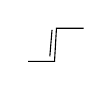
\begin{tikzpicture}[x=1em,y=1em]
\draw (0,0)--(.95,0)--(1.02,1.2)--(2,1.2);
\draw (.78,.18)--(.86,1.14);
\end{tikzpicture}}

Comme le \deleted{\unsure{sg}} premier de ces signes est forcément $\varepsilon'_1=\varepsilon_1$, cela signifie que \deleted{l'écriture} la suite de signes est la $=$ que celle des $\varepsilon_1,\varepsilon_2,\ldots,\unsure{\varepsilon_r,|\varepsilon_{r'}}$ (à la longueur près). Mais mieux, que l'expression $(\unsure{*})$ de $\tau'$ est son unique expression réduite, donc que $s=r'$ (longueur utile de $\tau'$), et que les $\lambda_i$ sont les longueurs $\ell'_i$ des intervalles critiques de $I_{\tau'}$.

\deleted{Cela signifie \deleted{\unsure{donc}} aussi que $F$ est \unsure{une composée|un composé} (par $*$) de morphismes \deleted{\unsure{d'intervalles de}} \inserted{des intervalles de} transition de $I_\tau$ \unsure{;} Si on désigne par}
\scanpage{349}
\mspage{88}
% archive sheet number: 348
\deleted{\unsure{Considér}} Soit donc $\alpha\in[1,s=r']$, et considérons la flèche \inserted{de tr.} $F$-critique $\underline{u}_{i_\alpha}$, soit $j_\alpha$ l'indice marquant l'intervalle critique \inserted{de $I_\tau$} contenant la \unsure{partie|portée} de $\underline{u}_{i_\alpha}$ de $I_\tau$
\[
\underline{u}_{i_\alpha}\in\mathrm{Fl}(I_{j_\alpha}),
\]
alors $F$ induit des morphismes \inserted{(croissants)} d'intervalles or.
\[
F_\alpha\doteq F|I_{j_\alpha}:I_{j_\alpha}\longrightarrow I'_\alpha
\]
et est trivial sur les autres intervalles critiques (ceux pas de la forme $I_{j_\alpha}$). \deleted{\unsure{Car $I_{j_\alpha}$. D'autre part, $F_\alpha$ n'est pas}} \inserted{La donnée des $F_\alpha$ détermine donc $F$} \deleted{\unsure{par recollage}} sur les $I_{j_\alpha}$, donc sur \uline{tous} les $I_{\unsure{j|i}}$, donc partout (par l'opération $*$ \deleted{\unsure{$\}$}} de composition par \unsure{recollement|accolement}). De plus \deleted{les $F_\alpha$} la condition a)
assurera que \deleted{les} \inserted{chaque} $F_\alpha$ \deleted{\unsure{sont}} de nature \inserted{assez} particulière~: une seule flèche de transition critique $\underline{u}_{i_\alpha}$. De plus, pour qu'on ait $F=F_0$, il faudra

b) \deleted{\unsure{La flèche de transition}} \inserted{$\forall\alpha\in[1,r']$} $\underline{u}_{i_\alpha}$ est la \uline{première} flèche de transition de l'intervalle critique $I_{j_\alpha}$ qui la contient.

Et enfin

c) La suite des intervalles critiques \deleted{\unsure{$I$}} de $I_\tau$
\[
I_{j_1},I_{j_2}\ldots I_{j_{r'}}\qquad(\text{de signes }\inserted{\text{alternés}}\ \varepsilon_1,-\varepsilon_1,\varepsilon_1,\ldots)
\]
associés aux flèches $F$-critiques, n'est autre que celle \deleted{des}
\[
I_1,I_2,\ldots I_{r'}
\]
des $r'$ premiers intervalles critiques de $I_\tau$, i.e. les
\[
(j_1,j_2,\ldots,j_{r'})=(1,2,\ldots,r').
\]
\scanpage{350}
\mspage{89}
% archive sheet number: 349
Ceci vu, l'idée naturelle pour ``déformer'' $F$ en $F_0$, c'est de trouver une suite d'homotopies qui transforment $F$ de façon à lui faire acquérir successivement les caractéristiques a), b), c) du voyageur pressé. \deleted{Pour} Au besoin, pour aller plus vite au but, on utilisera l'hypothèse de récurrence sur \deleted{\unsure{$n$}} \inserted{$n=\mathrm{long.}\,\tau$}, que le théorème \deleted{\unsure{est pr}} de connexité est \inserted{déjà} prouvé quand $I_{\unsure{\tau}}$ est de longueur \deleted{utile} $\leq n-1$. (NB Le \deleted{\unsure{est}} th. est trivial pour $\unsure{N|n|\tau}\leq1$, car alors les cat. $\underline{\mathrm{Hom}}_{\unsure{\varepsilon}}(\tau,\tau')$ sont \inserted{toutes ou bien} vides, ou bien ponctuelles)

\deleted{\unsure{Plusieurs} \deleted{\unsure{en}} étapes}

\deleted{1) Supposons qu'il y ait deux flèches \deleted{\unsure{de}} $F$-critique\unsure{s} consécutives \inserted{(dans la suite tot. ordonnée des fl. $F$-cr.)} de même signature, \deleted{\unsure{soient donc} $\underline{u}_k$ et $\underline{u}_\ell$ $(k<\ell)$, on va donc, par une suite de déformations, \unsure{désignons}} de $F$, qui \unsure{ne bougeront|en bougeant} $F$ \deleted{\unsure{pour}} sur les intervalles critiques $I_{k'},I_{\ell'}$ ($k'\leq\ell'$) qui contiennent $\underline{u}_k,\underline{u}_\ell$, et sur les éventuels \unsure{int. cr.} intermédiaires (si $k'<\ell'$), \deleted{mais pas sur les autres intervalles critiques, \unsure{coll}} Groupons ensemble toutes les flèches de tr. critiques d'une $=$ \deleted{\unsure{groupe de t}} \inserted{suite} maximale}
\deleted{\[
\deleted{\unsure{\underline{u}_{k},\underline{u}_{k+1},\ldots,\underline{u}_{k+t}}}
\inserted{\underline{u}_{i_\alpha},\underline{u}_{i_{\alpha+1}},\ldots,\underline{u}_{i_{\alpha+t}}}
\]}
\deleted{de \inserted{$t+1$} flèches critiques consécutives de $=$ signe $\varepsilon$ \unsure{(Et ex)|(Et soit}, c'est-à-dire que si $\alpha>1$, $\underline{u}_{i_{\alpha-1}}$ est de \deleted{\unsure{même signe que} $\varepsilon$,} \inserted{signe $-\varepsilon$,} et de $=$ si $\alpha+t<r'$, $\underline{u}_{i_{\alpha+t+1}}$ de signe $-\varepsilon$. \deleted{\unsure{Alors}} En regardant $p=\mathrm{source}\,\underline{u}_{i_\alpha}$, $q=\mathrm{but}\,\underline{u}_{i_{\alpha+t}}$, et le \unsure{sous-intervalle} $I=[p,q]$ de $I_\tau$, \deleted{\unsure{l'id}} si on \deleted{\unsure{n'a pas}} n'a pas $p=0$, $q=n$ ($=\mathrm{long}\,\tau$), l'hypothèse de récurrence, appliquée à $I$ (avec les signes induits par ceux de $I_\tau$) et à $I'=[f(p),f(q)]\subset I$, nous montre qu'on peut déformer $F$, \unsure{sauf|sans} toucher à}
\margin{$t\geq1$}
% Long tapered ink mark in lower left margin.
\figure{
\begin{tikzpicture}[x=1cm,y=1cm]
\fill (0,0) .. controls (.24,.36) and (.48,.78) .. (.51,1.05)
.. controls (.50,1.20) and (.64,1.19) .. (.62,1.02)
.. controls (.57,.75) and (.31,.28) .. (0,0);
\draw[gray,line width=1pt] (.03,.03) .. controls (.24,.28) and (.48,.62) .. (.55,.90);
\end{tikzpicture}}
\scanpage{351}
\mspage{\deleted{\unsure{89|80}}90}
% archive sheet number: 350
\deleted{\unsure{deux|aux} valeurs de $F$ en dehors de $I$ (donc des homotopies qui soient l'identité sur les sommets $s\in I_\tau\setminus I$, et de plus de \inserted{$p={}$}$0_I$ \deleted{\unsure{$*$}} et \inserted{$q={}$}$1_I$), en un $F'$ qui, sur $I$, n'aura qu'une seule flèche \inserted{de tr.} critique, et celle-ci $=$ \unsure{plus|p. ex.} au début, égale à $\underline{u}_{i_\alpha}$ (si on y tient).}

\deleted{Il faut cependant traiter à part le cas $p=0,q=n$. Alors les $\underline{u}_{i_\alpha}$ sont \uline{toutes} de $=$ signe, Et il s'agit d'homotoper $F$ à un foncteur $F'$ qui n'a qu'une seule flèche critique. \deleted{Si $\tau$ est \unsure{bien un} $\Delta_\varepsilon^n$, Si les $\underline{u}_{i_\alpha}$ ne \unsure{sont pas tous}, alors par l'hyp. de} récurrence on est ramené au cas, d'abord où sur chaque intervalle critique de $I_\tau$, il y a au plus une flèche critique. (il suffit de l'assurer sur le dernier intervalle critique, contenant la flèche $F$-critique $\underline{u}_n$), puis au cas où il n'y a que deux flèches critiques, \deleted{\unsure{et}} savoir $u_1$ et $u_n$. Ensuite, \deleted{on se ramène \unsure{encore} par l'hyp. de récurrence, en \unsure{ramenant} \unsure{un à à}} Utilisant l'hyp. de réc. pour $I=[1,n-1]\subset I_\tau$, etc \unsure{si on})}

1) On veut assurer a). Pour ceci, on utilisera l'hyp. de récurrence, pour \deleted{\unsure{grouper ensemble toutes les}} \inserted{remplacer un groupe \unsure{de au moins|de moins} $1$} flèches critiques consécutives de $=$ signe, par une seule flèche critique. \unsure{Ladite|cette} méthode ne foire que si les flèches critiques sont toutes de $=$ signe \inserted{$\varepsilon$} et \unsure{incluent|enclavent} $\underline{u}_1$ et $\underline{u}_n$. Mais l'hyp. de récurrence appliquée à $I=[1,n-1]\subset I_\tau$ nous ramène au cas où il n'y a que deux flèches critiques $u_1$ et $u_n$. Si le premier intervalle critique n'est pas réduit à $\Delta_\varepsilon$ i.e. est de longueur $2$, alors l'hyp. de récurrence appliquée à $\unsure{J|I}=[1,\unsure{n}]\subset I_\tau$ nous ramène au cas où les deux flèches critiques sont $\underline{u}_1$ et $\underline{u}_2$, \deleted{\unsure{donc alors}} \inserted{et on est}
\scanpage{352}
\mspage{91}
% archive sheet number: 351
alors ramené au cas où $\boxed{\unsure{I|\tau}=\Delta_\varepsilon^2}$\inserted{, $\tau'=\Delta_\varepsilon^2$}. Sinon, au cas \unsure{où|en} $\boxed{\tau=\Delta_\varepsilon\Delta_{-\varepsilon}^{\ell_2}\Delta_\varepsilon}$, \inserted{$\tau'=\Delta_\varepsilon^2$} et où \deleted{\unsure{une}} les deux flèches critiques sont encore la première et la dernière, et $\tau'=\Delta_\varepsilon^2$. Ce sont là les deux cas irréductibles, qu'il \deleted{\unsure{y}} faudra traiter \deleted{\unsure{de façon}} à part.

\deleted{2)} Ces cas admis, on a donc moyen pour déformer $F$ de façon à satisfaire a). \deleted{Soient} Ensuite, on veut

2) Assurer que la suite des intervalles critiques $I_{j_1},I_{j_2}\ldots I_{j_{r'}}$ qui \unsure{contient|contiennent} les flèches critiques $\underline{u}_{i_1},\ldots,\underline{u}_{i_{r'}}$, \deleted{\unsure{soit}} soit \unsure{de|la} suite $I_1,\ldots I_{r'}$.
C'est encore \unsure{immédiat$^{\mathrm{t}}$|immédiat} par l'hyp\unsure{.} de récurrence, le seul cas irréd. étant celui où $r'=1$\inserted{ (une seule flèche critique)}, et où il \deleted{\unsure{n'a que deux intervalles critiques, et}} s'agit de faire descendre cette flèche critique jusqu'à $\underline{u}_1$. Si $I_1$ est de longueur $>1$, alors on fait descendre en $\underline{u}_2$ par hyp. de récurrence, et le cas irréductible est celui où $\boxed{\tau=\Delta_\varepsilon^2}$\inserted{, $\tau'=\Delta_\varepsilon$} une flèche critique $\underline{u}_2$, la faire descendre en $\underline{u}_1$.

Si par contre $I_1$ de longueur $1$, le cas \unsure{irréductible} est $\boxed{\tau=\Delta_\varepsilon\Delta_{-\varepsilon}^{\ell_2}\Delta_\varepsilon}$, \deleted{la flèche} $\tau'=\Delta_\varepsilon$, une flèche critique $\underline{u}_{\ell_2+2}$, la faire descendre en $\underline{u}_1$.

Sous réserve de traiter ces \inserted{deux} nouveaux cas irréductibles, on peut déformer $F$ en un foncteur qui satisfait à a) et à c). Reste à normaliser chacun des $F_\alpha:I_\alpha\mathrel{\unsure{-|\to}}I'_\alpha$ ($\alpha\in[1,r']$).

Donc on est ramené à $\Delta_\varepsilon^{\unsure{n|N}}\longrightarrow\Delta_\varepsilon$~: \unsure{$\{$}une seule flèche critique\unsure{$\}$} $\underline{u}_\alpha$, $\alpha\in[1,n]$ $\}$, à faire descendre en $\underline{u}_{\deleted{\unsure{2}}\,\unsure{1}}$. Si $n\geq2$, par hyp. de récurrence elle descend \unsure{en} $\underline{u}_2$, cas supposé traité en $2^{\mathrm{o}}$). Donc
